\documentclass[11pt]{article}
\usepackage[margin=1in]{geometry}
% Preamble of tuning.tex: the packages, macros and figure palette of the math document
% (math.tex), plus the few symbols the tuning document adds. Needs pgfplots (docs/Dockerfile).
\usepackage[T1]{fontenc}
\usepackage{lmodern}
\usepackage{amsmath,amssymb,amsthm,bm}
\usepackage{booktabs}
\usepackage{array}
\usepackage{enumitem}
\usepackage{xcolor}
\usepackage{tikz}
\usetikzlibrary{arrows.meta,calc,positioning,decorations.pathreplacing,
  decorations.pathmorphing,patterns,shapes.geometric,fit}
\usepackage{pgfplots}
\pgfplotsset{compat=1.18}
\usepgfplotslibrary{groupplots}
\usepackage{caption}
\captionsetup{justification=raggedright, singlelinecheck=true}
\usepackage[hidelinks]{hyperref}

\newtheorem*{example}{Example}
\newcommand{\code}[1]{\texttt{\small #1}}
\newcommand{\file}[1]{\par\noindent{\small\raggedright\color{gray} Implemented in \texttt{#1}.\par}}
\newcommand{\ev}[1]{{\small\textsf{[#1]}}}          % an evidence citation: run, study row, session
\newcommand{\R}{\mathbb{R}}
\newcommand{\sgn}{\operatorname{sgn}}
\newcommand{\SD}{\operatorname{SD}}
\newcommand{\clip}{\operatorname{clip}}
\newcommand{\dd}{\mathrm{d}}
\newcommand{\nuv}{\bm{\nu}}                          % body velocity (u, v, r)
\newcommand{\dhat}{\hat{\bm d}}                      % world drift estimate, m/s
\newcommand{\Tl}{T}                                  % total lag tau + L

% --- figure colours (the math document's palette) -------------------------------
\definecolor{sA}{RGB}{31,119,180}     % blue: model / estimate / new method
\definecolor{sB}{RGB}{214,95,14}      % orange: alternative / old method / data
\definecolor{sC}{RGB}{44,140,60}      % green: accepted region / truth
\definecolor{sD}{RGB}{150,150,150}    % grey: guides


\title{Tuning Nav2 and the velocity loop on the MHSeals boat}
\author{\texttt{mhseals\_nav}, \texttt{mhseals\_hardware}, \texttt{mhseals\_testing}, \texttt{crane\_ml}}
\date{}

\begin{document}
\maketitle

\noindent This is the maths and the procedure behind every Nav2 and velocity-loop
parameter the boat runs with. Nav2's MPPI controller plans as if its command were the
boat's velocity. Everything between the command and the velocity (the velocity loop,
the thrusters, the hull and the odometry) is unmodelled by MPPI, so tuning is the job of
measuring that gap and turning each measured part into a limit, a gain or a gate. The
document follows one loop (Figure~\ref{fig:flow}): measure, classify, derive limits from
rules, tune for noise, gate behaviours, verify in simulation, decide. Each section ends with
the file that implements it. Every number cites its evidence in brackets: a study row of
the Python plant (\ev{plant\_v1:deadtime0.3}), a crane\_ml session
(\ev{tune\_A1\_pair}) or a mission batch. The companion \texttt{math.pdf} covers the
characterization, the mixer and the thrust model this document builds on.

\tableofcontents
\bigskip

\section{The tuning loop}
\label{sec:loop}

Nav2 and the velocity loop have been retuned many times. Every pass that worked followed
the same seven steps (Figure~\ref{fig:flow}); every pass that failed skipped one, usually by
tuning a symptom in Nav2 that belonged to the velocity loop, or by reading a sim win as a
boat win.

\begin{enumerate}[leftmargin=*, itemsep=2pt]
\item \textbf{Measure the plant and its latency} (Section~\ref{sec:latency},
  Section~\ref{sec:field}). Three boat sessions give everything: a Characterize run (its
  neutral phase gives the noise floor $\sigma_f$, its yaw onsets the dead time $L$, its yaw
  rows the rotation-centre offset $d$), Controller steps (the closed-loop lag $\tau$ per
  axis) and a moored log per GPS fix tier ($\sigma_p$). Mass, CoM and the antenna lever arm
  $l$ are bench numbers. The dead time comes from bags already recorded; no new run is
  needed to get it.
\item \textbf{Classify each difference} between the boat and the simulator
  (Section~\ref{sec:plant}). Steady plant differences (mass, drag, thrust scale, reverse
  ratio, a weak thruster) are absorbed by the velocity loop: they move route time by a few
  per cent. Delay and noise are not absorbed: delay drives yaw overshoot and noise drives
  shaking. Only those two, plus the geometry ($d$, $l$, $\sigma_p$), reach Nav2.
\item \textbf{Derive the limits from rules} (Section~\ref{sec:limits}). Each Nav2 velocity
  and acceleration limit is $\min(\text{measured}, \text{rule})$, where the rule keeps a
  stop inside a fixed distance and a turn's overshoot inside half the yaw tolerance, given
  the lag $T = \tau + L$. Goal tolerances come from the fix tier and the lever arm.
\item \textbf{Tune for noise robustness} (Section~\ref{sec:noise}). MPPI's temperature and
  sampling spreads decide how much a noisy odometry sample moves the plan; the velocity
  loop's $k_p$ decides how much it moves the thrusters. Each is set so the noise it passes on
  stays under half of what it would take to reverse something.
\item \textbf{Gate behaviours} (Section~\ref{sec:field}). Some conditions are not tuned around:
  docking only at RTK fixed, no tuning with a dead thruster, no start above 0.35\,m/s of
  drift, and latency fixed first when $L > 0.3$\,s.
\item \textbf{Verify in simulation} (Section~\ref{sec:verify}): crane\_ml runs of the
  candidate against the baseline over a matrix of plant variants and disturbances, scored by
  the motion-quality metrics of Section~\ref{sec:quality}.
\item \textbf{Decide by explicit thresholds} (Section~\ref{sec:accept}), set before the runs.
  A candidate that passes becomes a proposal to the owner, never a change on the boat.
\end{enumerate}

\noindent Two habits keep the loop honest. A change is attributed to one layer at a time:
the thruster chatter under odometry noise turned out to be the velocity loop's $k_p$, not
MPPI's (Section~\ref{sec:noise}), and the dock pin turned out to be the drift observer, not
the docking task (Section~\ref{sec:observer}). And a number is used only with its evidence:
the Python plant (\code{crane\_ml Tools/Tuning}) ranks causes quickly, but only a crane\_ml
full-stack run, with MPPI in the loop, confirms a Nav2 change.

\begin{figure}[tbp]
\centering
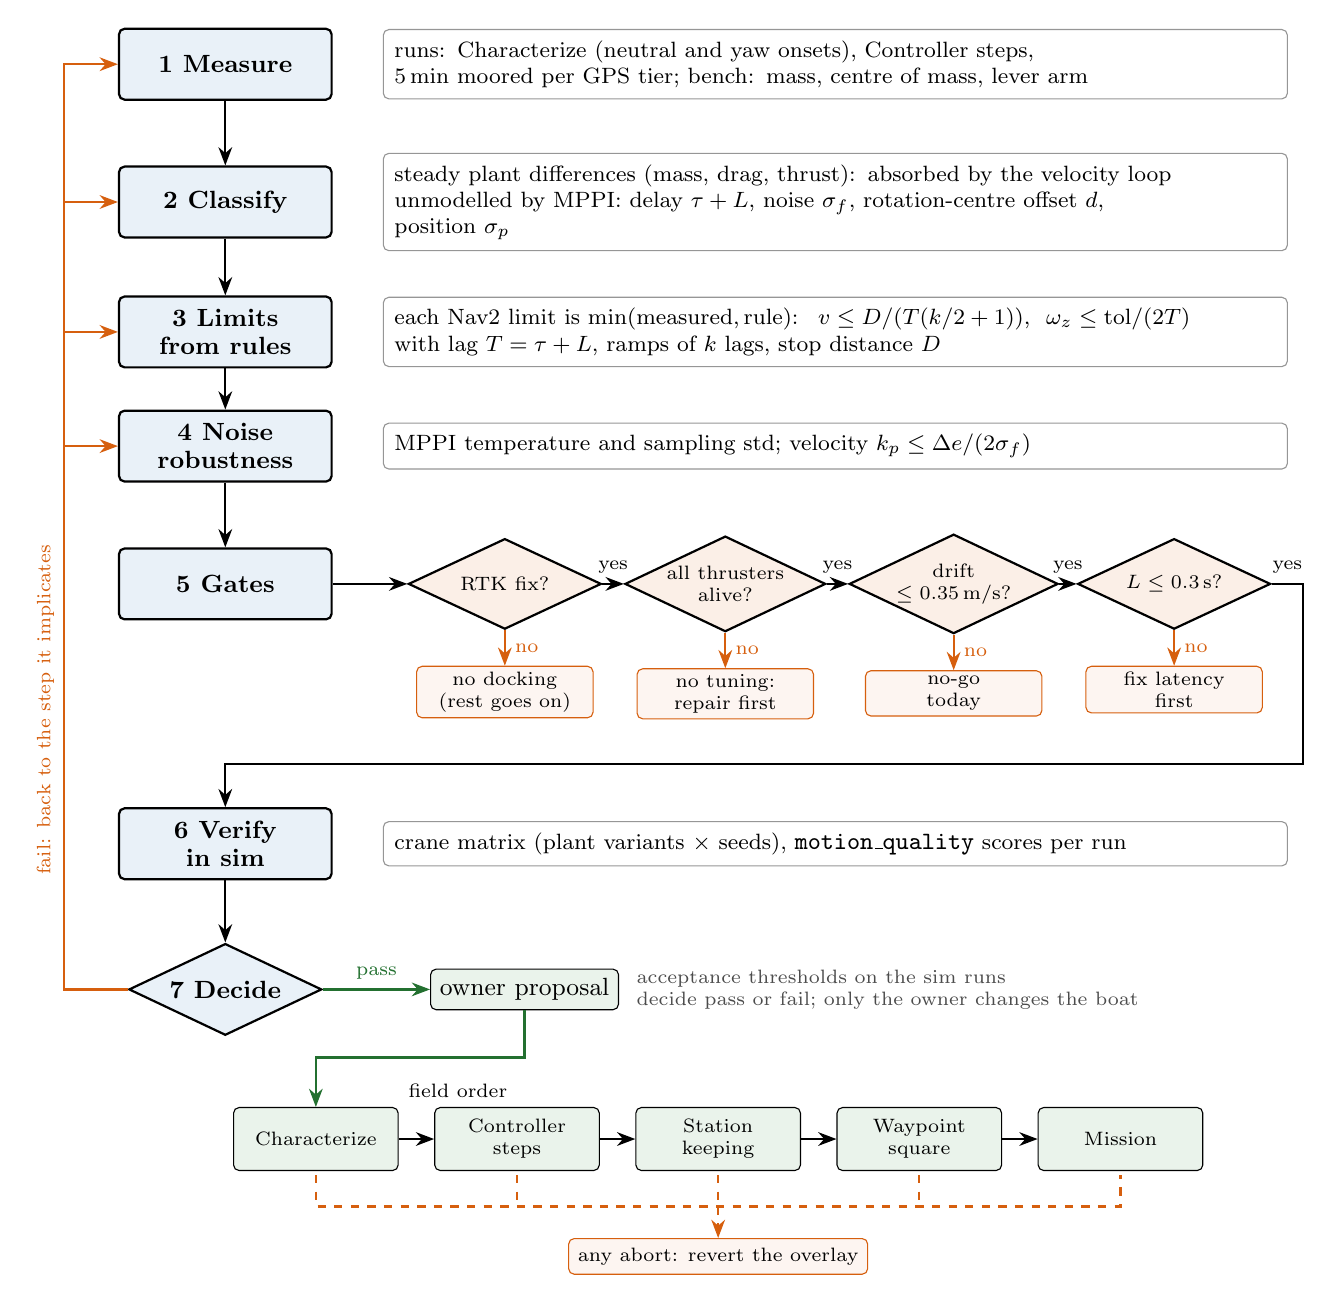
\begin{tikzpicture}[>=Stealth, font=\footnotesize,
  stage/.style={draw, thick, rounded corners=2pt, fill=sA!10, minimum width=2.7cm,
    minimum height=0.9cm, align=center, font=\small\bfseries},
  detail/.style={draw=sD, rounded corners=2pt, fill=white, text width=11.2cm, align=left,
    inner sep=4pt, anchor=west},
  gate/.style={draw, thick, diamond, aspect=2.1, fill=sB!10, align=center, inner sep=0.5pt,
    minimum width=2.45cm, minimum height=1.15cm,
    font=\scriptsize},
  stop/.style={draw=sB, rounded corners=2pt, fill=sB!6, align=center, font=\scriptsize,
    text width=2.1cm, inner sep=2pt},
  field/.style={draw, rounded corners=2pt, fill=sC!10, align=center, font=\scriptsize,
    minimum height=0.8cm, text width=1.95cm, inner sep=2pt},
  flow/.style={->, thick},
  back/.style={->, sB, thick}]
  % ---- the spine -------------------------------------------------------------------
  \node[stage] (measure)  at (0,0)     {1 Measure};
  \node[stage] (classify) at (0,-1.75) {2 Classify};
  \node[stage] (limits)   at (0,-3.4)  {3 Limits\\[-1pt]from rules};
  \node[stage] (noise)    at (0,-4.85) {4 Noise\\[-1pt]robustness};
  \node[stage] (gates)    at (0,-6.6)  {5 Gates};
  \node[stage] (verify)   at (0,-9.9)  {6 Verify\\[-1pt]in sim};
  \node[gate, font=\small\bfseries, fill=sA!10, aspect=1.6] (decide) at (0,-11.75) {7 Decide};
  \foreach \a/\b in {measure/classify, classify/limits, limits/noise, noise/gates}
    \draw[flow] (\a) -- (\b);
  % ---- what each step does ---------------------------------------------------------
  \node[detail] at (2.0,0) {runs: Characterize (neutral and yaw onsets), Controller steps,\\
    5\,min moored per GPS tier; bench: mass, centre of mass, lever arm};
  \node[detail] at (2.0,-1.75) {steady plant differences (mass, drag, thrust):
    absorbed by the velocity loop\\ unmodelled by MPPI: delay $\tau + L$,
    noise $\sigma_f$, rotation-centre offset $d$,\\ position $\sigma_p$};
  \node[detail] at (2.0,-3.4) {each Nav2 limit is $\min(\text{measured}, \text{rule})$:
    \ $v \le D / (T(k/2+1))$, \ $\omega_z \le \mathrm{tol}/(2T)$\\ with lag $T = \tau + L$, ramps of $k$ lags, stop distance $D$};
  \node[detail] at (2.0,-4.85) {MPPI temperature and sampling std; velocity
    $k_p \le \Delta e / (2\sigma_f)$};
  % ---- gates: a chain of checks, each with its own way out ---------------------------
  \node[gate] (g1) at (3.55,-6.6)  {RTK fix?};
  \node[gate] (g2) at (6.35,-6.6)  {all thrusters\\alive?};
  \node[gate] (g3) at (9.25,-6.6)  {drift\\$\le 0.35$\,m/s?};
  \node[gate] (g4) at (12.05,-6.6) {$L \le 0.3$\,s?};
  \draw[flow] (gates) -- (g1);
  \draw[flow] (g1) -- node[above, font=\scriptsize] {yes} (g2);
  \draw[flow] (g2) -- node[above, font=\scriptsize] {yes} (g3);
  \draw[flow] (g3) -- node[above, font=\scriptsize] {yes} (g4);
  \foreach \g/\txt in {g1/{no docking\\(rest goes on)}, g2/{no tuning:\\repair first},
                        g3/{no-go\\today}, g4/{fix latency\\first}} {
    \node[stop, below=0.45cm of \g] (s\g) {\txt};
    \draw[->, sB, thick] (\g) -- node[right, font=\scriptsize] {no} (s\g);
  }
  \draw[flow] (g4.east) -- node[above, font=\scriptsize] {yes} ++(0.4,0)
    |- ($(verify.north)+(0,0.55)$) -- (verify.north);
  \node[detail] at (2.0,-9.9) {crane matrix (plant variants $\times$ seeds),
    \code{motion\_quality} scores per run};
  \draw[flow] (verify) -- (decide);
  % ---- decide: pass -> owner and field order; fail -> back up the spine ------------
  \node[draw, rounded corners=2pt, fill=sC!10, align=center, font=\small, anchor=west]
    (owner) at (2.6,-11.75) {owner proposal};
  \node[anchor=west, font=\scriptsize, sD!50!black, align=left] at (5.1,-11.75)
    {acceptance thresholds on the sim runs\\ decide pass or fail; only the owner changes the boat};
  \draw[->, sC!80!black, thick] (decide) -- node[above, font=\scriptsize] {pass} (owner);
  \node[field] (f1) at (1.15,-13.65) {Characterize};
  \node[field, right=0.45cm of f1] (f2) {Controller\\steps};
  \node[field, right=0.45cm of f2] (f3) {Station\\keeping};
  \node[field, right=0.45cm of f3] (f4) {Waypoint\\square};
  \node[field, right=0.45cm of f4] (f5) {Mission};
  \foreach \a/\b in {f1/f2, f2/f3, f3/f4, f4/f5} \draw[flow] (\a) -- (\b);
  \draw[->, sC!80!black, thick] (owner.south) -- ++(0,-0.6) -| (f1.north);
  \node[font=\scriptsize, anchor=south west] at (f1.north east) {field order};
  \draw[sB, thick, dashed] ($(f1.south)+(0,-0.05)$) -- ++(0,-0.4) -| ($(f5.south)+(0,-0.05)$);
  \foreach \f in {f2,f3,f4} \draw[sB, thick, dashed] ($(\f.south)+(0,-0.05)$) -- ++(0,-0.4);
  \node[draw=sB, rounded corners=2pt, fill=sB!6, font=\scriptsize, below=0.85cm of f3] (revert) {any abort: revert the overlay};
  \draw[->, sB, thick, dashed] ($(f3.south)+(0,-0.45)$) -- (revert.north);
  % fail: a bus up the left side, back into the step the failure implicates
  \draw[back] (decide.west) -- (-2.05,-11.75) -- (-2.05,0) -- (measure.west);
  \foreach \s in {classify, limits, noise} \draw[back] (-2.05,0 |- \s) -- (\s.west);
  \node[sB, font=\scriptsize, rotate=90, anchor=south] at (-2.05,-8.2)
    {fail: back to the step it implicates};
\end{tikzpicture}
\caption{The tuning loop and the spine of this document. Steps 1--4 turn measurements
into limits and gains; the gates (diamonds) stop or narrow a session before any
tuning; step~6 runs the candidate through the simulated plant matrix and step~7
compares it with the acceptance thresholds. A pass becomes an owner proposal that the
boat then tests in the field order, and any abort reverts the overlay. A fail goes back to
the step it implicates.}
\label{fig:flow}
\end{figure}


\section{The plant and what its differences do}
\label{sec:plant}

\subsection{The 3-DOF model}
The hull moves in surge $u$, sway $v$ and yaw rate $r$, in the body frame (x forward, y
port) with the origin at the centre of mass. A constant world current $\bm c$ makes the
water-relative velocity the one the hydrodynamics see,
\[
  \nuv_r = \nuv - \begin{bmatrix} R(\psi)^\top \bm c \\ 0 \end{bmatrix},
  \qquad
  M\dot{\nuv}_r + C(\nuv_r)\,\nuv_r + D(\nuv_r)\,\nuv_r = \bm\tau_\text{thr} + \bm\tau_\text{env},
\]
with
\[
  M = \operatorname{diag}(m + a_u,\; m + a_v,\; I_z + a_r),\qquad
  C(\nuv_r) = \begin{bmatrix} 0 & 0 & -M_{22} v_r \\ 0 & 0 & M_{11} u_r \\ M_{22} v_r & -M_{11} u_r & 0 \end{bmatrix},
\]
and a linear-plus-quadratic damping per axis, $D(\nuv_r)\nuv_r = (D_{1j} + D_{2j}|\nu_j|)\,\nu_j$.
The rigid body may integrate in $\nuv_r$ because its Coriolis term does not depend on the
linear velocity. The $(3,\cdot)$ row of $C$ gives the Munk moment $-(M_{22}-M_{11})\,u_r v_r$:
with sway added mass much larger than surge's, a hull moving obliquely is turned broadside.
The added-mass priors are $a_u = 5.5 \pm 2.8$\,kg, $a_v = 21.3$\,kg and $a_r \approx 2.4$\,kg\,m$^2$
\ev{sim2real R1-2}; the nominal plant (crane\_ml's physics: $m = 30$\,kg, $I_z = 4.1$\,kg\,m$^2$,
no added mass) is a fixture, not a measurement of the boat.

\paragraph{The thrust map.} Thruster $i$ at $(x_i, y_i)$ pushes along a unit vector at mount
angle $\alpha_i$ (45$^\circ$ mounts; $|x_i| = 0.266$, $|y_i| = 0.343$\,m, a yaw lever of 0.43\,m).
Its column of the wrench matrix, about the CoM, is
\[
  \bm b_i = \begin{bmatrix} \cos\alpha_i \\ \sin\alpha_i \\ x_i \sin\alpha_i - y_i\cos\alpha_i \end{bmatrix},
  \qquad
  \bm\tau_\text{thr} = \sum_i \bm b_i\, f_i,
\]
so a lever $y$ contributes $-y X$ to the yaw moment \ev{sim2real R3-8, corrected sign}. The thrust of an effort
$e \in [-1,1]$ is quadratic in the effort outside the ESC deadband $\delta$:
\[
  f_i = F^{\sgn e}\,\Big(\frac{|e| - \delta}{1 - \delta}\Big)_+^2 \sgn e ,
  \qquad F^{+} = 51.5\text{\,N},\; F^{-} = 40.2\text{\,N (T200)},\; \delta = \tfrac{25}{400} = 0.0625,
\]
reached through a first-order spool (time constant 0.1\,s) after any pure dead time. The
thrust grows as $e|e|$: every wrench curve is in $e|e|$, never in $e$. The per-thruster forward
and reverse scale is measured on the bench by pair pulls (\texttt{bench.pdf}), not fitted
from motion.

\paragraph{The speed curves.} In steady motion along one axis the wrench balances the drag,
$F_j\, e|e| = D_{1j} v + D_{2j} v|v|$, so the velocity loop's model of each axis and sign is
\[
  e|e| = d_1 v + d_2 v|v|,\qquad d_1 = D_1/F,\; d_2 = D_2/F,
\]
fitted by the characterization (\texttt{math.pdf}). It is monotone for $d_1 \ge 0$ and
$d_1 + 2 d_2 v_\text{max} > 0$, and inverts in closed form. A fit done in effort form clamps
$d_2$ to 0. Section~\ref{sec:vlaw} inverts these curves; nothing in this document uses a
straight-line gain.
\file{crane\_ml Tools/Tuning/plant.py (fixture plant); mhseals\_hardware velocity\_law.Plant (curves)}

\subsection{Classifying the differences}
\label{sec:classify}
The Python plant (\code{plant.py}) runs the boat's own velocity law and mixer, imported
unchanged, behind a Nav2-like command layer (\code{loop.py}). Each study row is one plant
variant and seed, with the route, a step and a carved turn scored; the rows carry the
variant, the limits and the git heads (\code{study.py}). Varying one thing at a time sorts the
differences into four kinds (Table~\ref{tab:classify}).

\begin{table}[h]
\centering\small
\begin{tabular}{@{}p{0.36\linewidth}p{0.36\linewidth}p{0.2\linewidth}@{}}
\toprule
Difference & Effect at today's limits (0.4\,m/s, 0.3\,rad/s) & Reaches \\
\midrule
\textbf{Steady plant}: mass 19--40\,kg, added mass, $I_z$ 2--8, drag $\times$0.6--1.6, thrust $\times$0.7,
sag 0.8, reverse ratio 0.6, one thruster at 80\%, mount error 8$^\circ$ \ev{plant\_v1}
& absorbed: route time $\pm$3\%, peak effort $\le 0.56$; the lag $\tau$ grows (surge 0.25$\to$0.45\,s,
sway 0.3$\to$0.75\,s) & $\tau$ only \\
\addlinespace
\textbf{Delay}: dead time 0.15 / 0.3\,s, odometry latency 0.25\,s \ev{plant\_v1:deadtime*, disturb\_v1:latency0.25}
& yaw overshoot 40\% / 82\%; yaw reversals 2.2$\to$9.5\,/min; 8\,/min at 0.25\,s latency & $w_z$, $\alpha_z$, rotate speed \\
\addlinespace
\textbf{Noise}: odometry velocity SD 0.05 / 0.12\,m/s, waves 0.12\,m/s \ev{disturb\_v1:velnoise*, waves0.12}
& thruster reversals 31 / 152\,/min; waves: yaw reversals 17\,/min & $k_p$, MPPI noise keys \\
\addlinespace
\textbf{Geometry}: CoM 0.10\,m from base\_link; GPS $\sigma$ 0.5 / 1.5\,m (float) \ev{ad hoc runs t3/t5; disturb\_v1:gps*}
& base\_link walks 0.16\,m per in-place 180$^\circ$; hold RMS 0.6 / 2.3\,m & goal tolerances \\
\bottomrule
\end{tabular}
\caption{The four kinds of boat-to-sim difference and the parameters each one reaches.
Python plant: \code{plant\_v1} rows are seed 0 only (one per variant); \code{disturb\_v1} rows are
means of seeds 0--2, as are all other Python-plant study numbers in this document.}
\label{tab:classify}
\end{table}

\noindent The steady differences need no Nav2 change because the velocity loop's feed-forward
and integral take them up; they matter only through the lag $\tau$ that the rules of
Section~\ref{sec:limits} read. Two more rows are gates rather than tuning: one dead thruster
still completes the route but overshoots goals by 0.77\,m \ev{disturb\_v1:FL\_dead}, and a
9\,m/s wind overshoots by 1.35\,m because the observer takes wind for current
\ev{disturb\_v1:wind9\_ne}.

\section{The velocity loop and the drift observer}
\label{sec:vlaw}

Nav2 sends a body velocity; the boat's velocity law turns it into effort
(Figure~\ref{fig:loop}). Whatever this loop does between the command and the velocity is what
MPPI does not model, so it is tuned first and read by every later rule.

\begin{figure}[tbp]
\centering
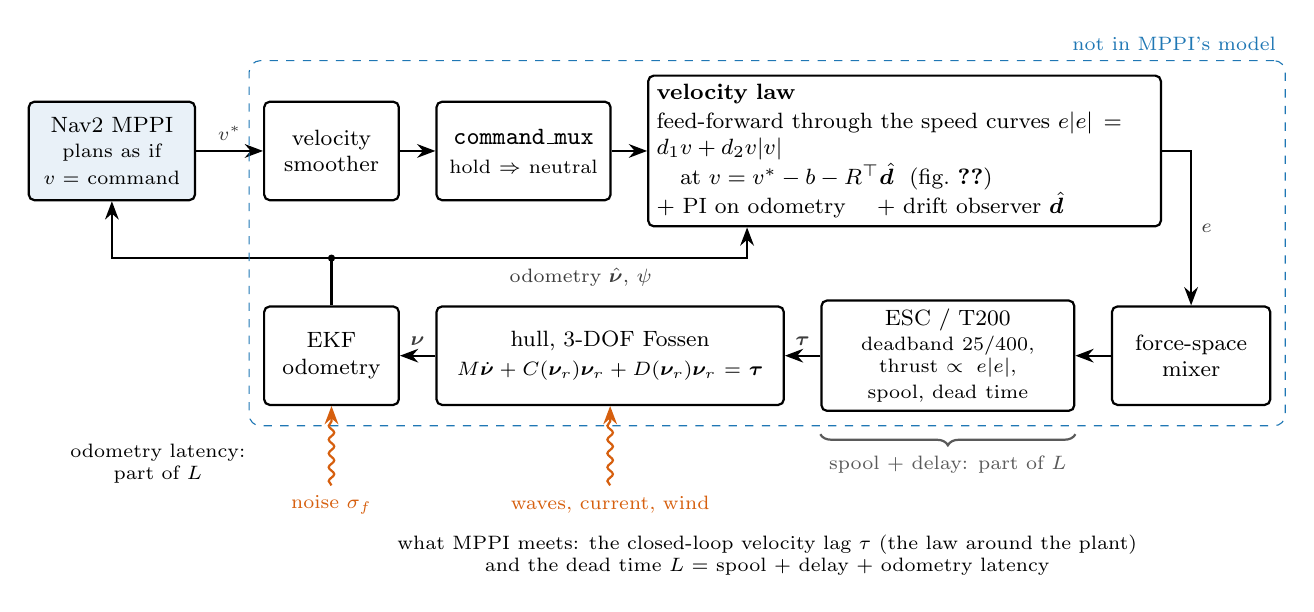
\begin{tikzpicture}[>=Stealth, font=\footnotesize,
  blk/.style={draw, thick, rounded corners=2pt, fill=white, align=center, inner sep=3pt,
    minimum height=1.25cm},
  sub/.style={font=\scriptsize, sD!40!black},
  sig/.style={->, thick},
  dist/.style={->, thick, sB, decorate, decoration={snake, amplitude=1pt, segment length=5pt,
    post length=4pt}},
  note/.style={font=\scriptsize, align=center}]
  % ---- top row: command path ---------------------------------------------------------
  \node[blk, fill=sA!10, text width=1.9cm] (mppi) at (0,0)
    {Nav2 MPPI\\[1pt] {\scriptsize plans as if\\ $v = $ command}};
  \node[blk, text width=1.5cm, right=0.85cm of mppi] (smooth) {velocity\\smoother};
  \node[blk, text width=2.0cm, right=0.45cm of smooth] (mux)
    {\code{command\_mux}\\[1pt] {\scriptsize hold $\Rightarrow$ neutral}};
  \node[blk, text width=6.3cm, right=0.45cm of mux, align=left] (law)
    {\textbf{velocity law}\\[1pt]
     feed-forward through the speed curves $e|e| = d_1 v + d_2 v|v|$\\
     \quad at $v = v^* - b - R^\top\dhat$ \ (fig.~\ref{fig:observer})\\
     $+$ PI on odometry \quad $+$ drift observer $\dhat$};
  % ---- bottom row: plant path, right to left ----------------------------------------
  \node[blk, text width=1.5cm] (ekf) at ($(smooth)+(0,-2.6)$) {EKF\\odometry};
  \node[blk, text width=4.2cm, right=0.45cm of ekf] (hull)
    {hull, 3-DOF Fossen\\[1pt] {\scriptsize $M\dot\nuv + C(\nuv_r)\nuv_r + D(\nuv_r)\nuv_r = \bm\tau$}};
  \node[blk, text width=3.0cm, right=0.45cm of hull] (esc)
    {ESC / T200\\[1pt] {\scriptsize deadband 25/400, thrust $\propto e|e|$,\\ spool, dead time}};
  \node[blk, text width=1.8cm, right=0.45cm of esc] (mixer) {force-space\\mixer};
  % ---- signals ------------------------------------------------------------------------
  \draw[sig] (mppi) -- node[above, sub] {$v^*$} (smooth);
  \draw[sig] (smooth) -- (mux);
  \draw[sig] (mux) -- (law);
  \draw[sig] (law.east) -| node[pos=0.75, right, sub] {$e$} (mixer.north);
  \draw[sig] (mixer) -- (esc);
  \draw[sig] (esc) -- node[above, sub] {$\bm\tau$} (hull);
  \draw[sig] (hull) -- node[above, sub] {$\nuv$} (ekf);
  \coordinate (fb) at ($(ekf.north)+(0,0.6)$);
  \draw[thick] (ekf.north) -- (fb);
  \draw[sig] (fb) -| (mppi.south);
  \draw[sig] (fb) -| node[pos=0.3, below, sub] {odometry $\hat\nuv$, $\psi$} ($(law.south)+(-2.0,0)$);
  \fill (fb) circle (1.3pt);
  % ---- what MPPI does not model --------------------------------------------------------
  \node[draw=sA, dashed, rounded corners=4pt, inner sep=5pt,
    fit=(smooth) (mux) (law) (mixer) (esc) (hull) (ekf)] (gap) {};
  \node[anchor=south east, sA, font=\scriptsize] at (gap.north east) {not in MPPI's model};
  % ---- what enters from outside, and where the lag comes from ---------------------------
  \draw[dist] ($(hull.south |- gap.south)+(0,-0.75)$) node[below, note, sB] {waves, current, wind}
    -- (hull.south);
  \draw[dist] ($(ekf.south |- gap.south)+(0,-0.75)$) node[below, note, sB] {noise $\sigma_f$}
    -- (ekf.south);
  \draw[decorate, decoration={brace, amplitude=4pt, mirror}, thick, sD!60!black]
    ($(esc.west |- gap.south)+(0,-0.1)$) -- ($(esc.east |- gap.south)+(0,-0.1)$)
    node[midway, below=4pt, note] {spool + delay: part of $L$};
  \node[note, anchor=north east] at ($(ekf.west |- gap.south)+(-0.1,-0.1)$) {odometry latency:\\ part of $L$};
  \node[note, anchor=north] at ($(gap.south)+(0,-1.25)$)
    {what MPPI meets: the closed-loop velocity lag $\tau$ (the law around the plant)\\
     and the dead time $L$ = spool + delay + odometry latency};
\end{tikzpicture}
\caption{The velocity loop between Nav2 and the water. MPPI plans as if the boat moved
at the commanded velocity; everything inside the dashed box is outside its model. The
velocity law closes a loop around the thrusters and the hull: its feed-forward inverts
the per-direction speed curves at the wanted velocity less the mechanical bias $b$ and
the drift estimate $\dhat$ rotated into the body, and PI feedback on odometry covers the
rest. What MPPI sees of that box is a lag $\tau$, a dead time $L$, the odometry noise
$\sigma_f$ and the disturbances acting on the hull. A hold in \code{command\_mux} sends
neutral thrust, not station keeping.}
\label{fig:loop}
\end{figure}


\subsection{The law}
Let $\bm v^\star = \clip(\bm v^*, -\bm v_\text{max}, \bm v_\text{max})$ be the clipped request,
$\bm b$ the body-fixed mechanical bias, $\dhat$ the world drift estimate and $s_j^{-1}$ the
inverse of axis $j$'s speed curve, $s_j^{-1}(v) = \sgn(w)\sqrt{|w|}$ with $w = d_1 v + d_2 v|v|$.
Per axis,
\[
  e_j = \clip\!\Big(\underbrace{s_j^{-1}\big(v^\star_j - b_j - [R(\psi)^\top\dhat]_j\big)}_{\text{feed-forward}}
        + k_{p,j}\,\epsilon_j + k_{i,j}\,z_j,\; -1,\; 1\Big),
  \qquad \epsilon_j = v^\star_j - v_j ,
\]
with the integral $z_j$ clipped to $\pm z_\text{max}$ (\code{integral\_limit}) and frozen on an
axis pinned at $\pm1$ in the direction of its error (conditional integration). The
defaults are $k_p = (0.8, 0.8, 0.6)$, $k_i = (0.6, 0.6, 0.4)$, $z_\text{max} = 0.3$.

\paragraph{Why invert the curve, and not a gain.} The feed-forward is exact on the model, so
the PI loop only meets what the model gets wrong. A straight-line gain would leave the loop a
speed-dependent error, and a correction through the \emph{secant} gain of a power law
over-corrects: for $y = c\,x^n$ the secant inverse gives $\Delta x = \Delta y\,x/y$, $n$ times
the local inverse $\Delta y/(n c x^{n-1})$. So no measured lag or offset is ``undone'' by
dividing by a secant gain; the curve is inverted, and the residual is left to feedback.

\paragraph{The integral ceiling.} $z_\text{max}$ bounds what the integral can hold. With the
observer off (a stale estimate) it binds only from about 0.45\,m/s of current: goal overshoot
0.39\,m at $z_\text{max} = 0.3$ against 0.27\,m at 0.5 in a 0.45\,m/s current, and no gain at
0.3\,m/s (0.19 against 0.21\,m) \ev{stale\_v1:stale\_il0.3\_c0.45, stale\_il0.5\_c0.45, stale\_il0.3, stale\_il0.5}.
Raising it is optional and only for currents over 0.45\,m/s.
\file{mhseals\_hardware/velocity\_law.py (VelocityLaw.step)}

\subsection{The drift observer}
\label{sec:observer}
Current and wind change from day to day, so the drift is estimated on the boat, in the world
frame where it is constant, and rotated into the body when used. Each odometry sample gives
the part of the velocity the model cannot explain,
\[
  \bm\rho = R(\psi)\,\big(\bm v - \bm b - \bm s(\bm e)\big)_{xy},
\]
and a first-order filter with $\alpha = \Delta t/(\tau_d + \Delta t)$, $\tau_d = 5$\,s, averages it:
$\dhat \leftarrow \dhat + \alpha(\bm\rho - \dhat)$. Three rules decide when it may learn
(Figure~\ref{fig:observer}).

\begin{description}[leftmargin=1em, itemsep=2pt]
\item[Only at rest.] It learns only while every $|v^\star_j| \le 0.1$ (\code{drift\_command\_limit})
  and no effort is saturated. Under way, $\bm\rho$ is mostly the model's own error, which would
  be taken for current and turned with the boat; the estimate is held and the PI covers the
  rest. A held estimate matters: with the observer off, skid in a carved turn in a 0.3\,m/s
  cross-current doubles, 0.054$\to$0.107\,m/s \ev{stale\_v1:observer\_on\_il0.3, stale\_il0.3}.
\item[The sign gate.] Against a dock or a buoy the boat stops while the effort pushes on. The
  residual then reads as a current pushing it \emph{off} the contact, and learning it would
  hold the push and add to it every cycle. A real current that is not yet compensated does the
  opposite: it carries the boat \emph{along} the residual before the loop catches it. So the
  observer integrates the world displacement since the boat last got under way,
  $\bm q \leftarrow \bm q + \Delta t\,R(\psi)\bm v_{xy}$ (on learning samples; reset to 0 whenever
  under way), and lets $|\dhat|$ grow only once
  \[
    \bm q\cdot\frac{\bm\rho}{|\bm\rho|} > q_\text{min} = 0.02\text{\,m}\quad(\code{drift\_carry});
  \]
  otherwise the update may shrink or turn the estimate but $|\dhat|$ is capped at its previous
  size. The gate reads displacement, not speed, because the PI loop soon stops a drifting boat:
  the carry it already had stays on record. The correction is sign-dependent by construction:
  being carried along the residual opens the gate; reaching the dock moving the other way, or
  being pinned, keeps it shut.
\item[The cap.] $|\dhat| \le d_\text{max} = 0.5$\,m/s (\code{drift\_limit}) always: no current
  the boat operates in is faster, and the cap bounds the damage of any path the gate misses. It
  must stay well below the slowest axis's full-effort speed (usually sway), or the feed-forward
  alone could still drive that axis to full effort against a contact.
\end{description}

\noindent The failure these rules remove was seen in crane\_ml's full mission: in the dock
back-out the command stayed under 0.1\,m/s, the observer learned the dock contact as current,
and the effort wound up to $(-0.8, +1.0)$ and pinned the boat to the tine until Nav2 reported
no progress \ev{ma\_v3 seed 2}. The estimate exceeded 0.35\,m/s for 10\,s or more in a
0.15\,m/s current \ev{ma\_v2 seed 0}.

\begin{figure}[tbp]
\centering
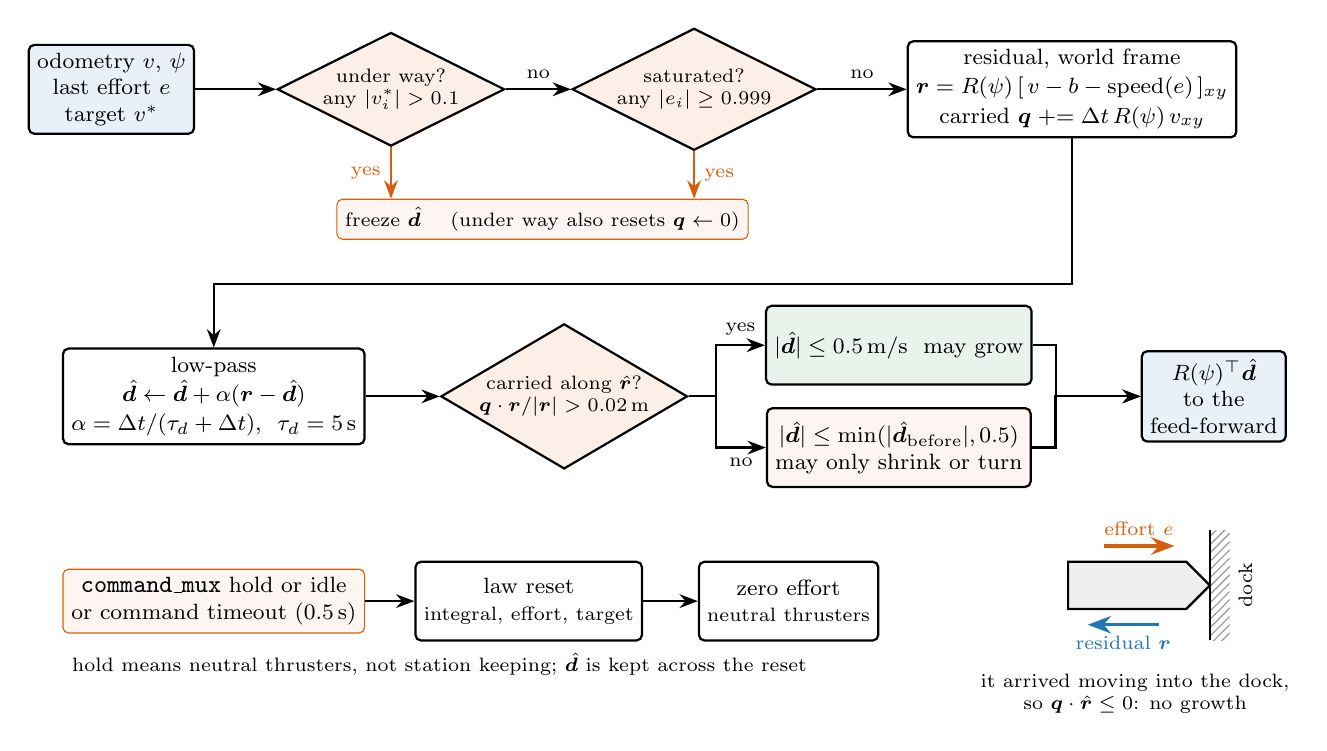
\begin{tikzpicture}[>=Stealth, font=\footnotesize,
  blk/.style={draw, thick, rounded corners=2pt, fill=white, align=center, inner sep=3pt,
    minimum height=1.0cm},
  gate/.style={draw, thick, diamond, aspect=2.0, fill=sB!10, align=center, inner sep=0.5pt,
    font=\scriptsize},
  frz/.style={draw=sB, rounded corners=2pt, fill=sB!6, align=center, font=\scriptsize,
    inner sep=3pt},
  sig/.style={->, thick},
  lab/.style={font=\scriptsize}]
  % ---- row 1: when the observer may learn --------------------------------------------
  \node[blk, fill=sA!10] (in) at (0,0) {odometry $v$, $\psi$\\ last effort $e$\\ target $v^*$};
  \node[gate] (way) at (3.55,0) {under way?\\ any $|v^*_i| > 0.1$};
  \node[gate] (sat) at (7.4,0) {saturated?\\ any $|e_i| \ge 0.999$};
  \node[blk] (res) at (12.2,0)
    {residual, world frame\\[1pt]
     $\bm r = R(\psi)\,[\,v - b - \mathrm{speed}(e)\,]_{xy}$\\[1pt]
     carried $\bm q \mathrel{+}= \Delta t\, R(\psi)\,v_{xy}$};
  \draw[sig] (in) -- (way);
  \draw[sig] (way) -- node[above, lab] {no} (sat);
  \draw[sig] (sat) -- node[above, lab] {no} (res);
  \node[frz] (freeze) at (5.475,-1.65) {freeze $\dhat$ \quad (under way also resets $\bm q \leftarrow 0$)};
  \draw[->, sB, thick] (way.south) -- node[left, lab] {yes} (way.south |- freeze.north);
  \draw[->, sB, thick] (sat.south) -- node[right, lab] {yes} (sat.south |- freeze.north);
  % ---- row 2: low-pass, then the sign gate, then the cap ----------------------------
  \node[blk] (lp) at (1.3,-3.9)
    {low-pass\\[1pt] $\dhat \leftarrow \dhat + \alpha(\bm r - \dhat)$\\[1pt]
     $\alpha = \Delta t / (\tau_d + \Delta t)$, \ $\tau_d = 5$\,s};
  \node[gate, aspect=1.7] (sign) at (5.75,-3.9) {carried along $\hat{\bm r}$?\\
    $\bm q \cdot \bm r / |\bm r| > 0.02$\,m};
  \node[blk, fill=sC!10] (grow) at (10.0,-3.25) {$|\dhat| \le 0.5$\,m/s \ may grow};
  \node[blk, fill=sB!6] (keep) at (10.0,-4.55) {$|\dhat| \le \min(|\dhat_{\text{before}}|, 0.5)$\\
    may only shrink or turn};
  \node[blk, fill=sA!10] (out) at (14.0,-3.9) {$R(\psi)^\top \dhat$\\ to the\\ feed-forward};
  \draw[sig] (res.south) -- ++(0,-1.85) -| (lp.north);
  \draw[sig] (lp) -- (sign);
  \draw[sig] (sign.east) -- ++(0.35,0) |- node[pos=0.75, above, lab] {yes} (grow.west);
  \draw[sig] (sign.east) -- ++(0.35,0) |- node[pos=0.75, below, lab] {no} (keep.west);
  \draw[sig] (grow.east) -- ++(0.3,0) |- (out.west);
  \draw[sig] (keep.east) -- ++(0.3,0) |- (out.west);
  % ---- row 3: the side path that bypasses the law -------------------------------------
  \node[frz, font=\footnotesize] (hold) at (1.3,-6.5) {\code{command\_mux} hold or idle\\ or command timeout (0.5\,s)};
  \node[blk] (reset) at (5.3,-6.5) {law reset\\ {\scriptsize integral, effort, target}};
  \node[blk] (zero) at (8.6,-6.5) {zero effort\\ {\scriptsize neutral thrusters}};
  \draw[sig] (hold) -- (reset);
  \draw[sig] (reset) -- (zero);
  \node[lab, align=left, anchor=north west] at ($(hold.south west)+(0,-0.12)$)
    {hold means neutral thrusters, not station keeping; $\dhat$ is kept across the reset};
  % ---- inset: the boat pinned on a dock -------------------------------------------------
  \begin{scope}[shift={(12.9,-6.3)}]
    \fill[pattern=north east lines, pattern color=sD] (1.05,-0.7) rectangle (1.3,0.7);
    \draw[thick] (1.05,-0.7) -- (1.05,0.7);
    \node[lab, rotate=90] at (1.5,0) {dock};
    \draw[thick, fill=sD!15] (-0.75,-0.3) -- (0.75,-0.3) -- (1.05,0) -- (0.75,0.3) -- (-0.75,0.3) -- cycle;
    \draw[->, very thick, sB] (-0.3,0.5) -- node[above, lab] {effort $e$} ++(0.9,0);
    \draw[->, very thick, sA] (0.4,-0.5) -- node[below, lab] {residual $\bm r$} ++(-0.9,0);
    \node[lab, align=center, anchor=north] at (0.1,-1.0) {it arrived moving into the dock,\\ so $\bm q \cdot \hat{\bm r} \le 0$: no growth};
  \end{scope}
\end{tikzpicture}
\caption{The drift observer of the velocity law (\code{mhseals\_hardware} \code{velocity\_law.py}).
It learns only while the boat is asked to hold still and no axis is saturated: the
residual $\bm r$, the body velocity the speed curves do not explain, is turned into the
world frame and low-passed into $\dhat$ with $\tau_d = 5$\,s. The estimate may grow only
once the boat has been \emph{carried} at least 2\,cm along $\bm r$ since it last got under
way; otherwise it may only shrink or turn, and $|\dhat| \le 0.5$\,m/s always. Inset: a
boat pushed against a dock reads its stalled effort as a current pushing it off the
contact, but it reached the contact moving the other way, so the estimate does not grow and the push
does not wind up. Constants: \code{drift\_command\_limit} 0.1, \code{drift\_time\_constant}
5\,s, \code{drift\_carry} 0.02\,m, \code{drift\_limit} 0.5\,m/s.}
\label{fig:observer}
\end{figure}


\paragraph{Hold means neutral.} The controller follows the command mux's latched state: while
its input is anything but auto, manual or RC (a hold, including the operator's \texttt{E}, or idle),
or the state cannot be read, the law is reset and the effort is zero. The command timeout does
the same. The mux sends zeros while it holds; without this the law would station-keep on them,
with the drift feed-forward and the kept integral still pushing. Station
keeping happens only when autonomy explicitly commands zero velocity; a hold never drives the
thrusters to hold position. The remote e-stop is separate: it cuts thruster power in hardware
and is latched until the arm flow re-enables it.

\paragraph{Drift as a gate.} Because the estimate is held under way, a large estimate at the
start of a task is a condition, not a parameter: above 0.35\,m/s precise tasks (docking) do not
start (Section~\ref{sec:field}).
\file{mhseals\_hardware/velocity\_law.py (VelocityLaw.observe), velocity\_controller.py (hold, reset)}

\section{Latency: the lag MPPI does not see}
\label{sec:latency}

\subsection{The model}
Between a command and the odometry that shows its effect sit three delays in series: the pure
delay of the command chain $L_d$ (pulse out, ESC), the thruster spool (first order, time
constant $\tau_s$) and the odometry latency $L_o$ (EKF and transport); then the hull itself
responds with time constant $\tau_h$ ($I_z$ over the linearized damping, for yaw). Seen from
the odometry, a yaw onset from rest is close to a first-order-plus-dead-time (FOPDT)
response,
\[
  r(t) = r_0 + K\Big(1 - e^{-(t - t_\text{on} - L)/\tau}\Big)\quad (t > t_\text{on} + L),
  \qquad r(t) = r_0 \text{ before},
\]
with the apparent dead time
\[
  L \approx L_d + L_o + c\,\tau_s, \qquad c \approx \tfrac12,
\]
since a FOPDT fit of a two-lag cascade moves about half the smaller lag into the dead time
(Skogestad's half rule). On synthetic onsets the fit recovered $L_d + L_o$ within $\pm0.01$\,s,
with $c$ between 0.40 and 0.50 \ev{latency synthetic, 16 cases}. That $L$ is what the loop
feels, so it is the right input to the rules; the closed-loop velocity lag $\tau$ per axis is
measured separately by Controller steps as the 10--90\% rise time over $\ln 9$ (the rise time
of a first-order response is $\tau\ln 9$). The total lag of axis $a$ is
\[
  T_a = \tau_a + L .
\]

\subsection{The fit}
Onsets are pulse outputs that leave neutral ($|p - 1500| \ge 25\,\mu$s on any thruster) after at
least 1\,s of rest. For each onset the yaw rate over $[-0.5, 3]$\,s is fitted on a grid of
$(L, \tau)$, $L \in [0, 0.8]$\,s by 0.01, $\tau \in [0.04, 1.5]$\,s by 0.02, with $r_0$ and $K$ solved
by least squares at each node. An onset says nothing, and is dropped, when $|K|$ is under four
times the pre-onset noise or the optimum sits on the grid's edge. The result is the median $L$
over onsets with a bootstrap 90\% interval (2000 resamples, seed 0).

Yaw is used because its $\tau_h$ is the shortest (0.1--0.3\,s), which separates it best from $L$,
and the gyro is the cleanest channel. Both series are bag receipt times on the boat computer,
so no clock alignment enters.

\paragraph{Acceptance.} At least 6 fitted onsets and a 90\% interval no wider than 0.05\,s;
otherwise one more Characterize yaw pair (it runs both signs).

\paragraph{Evidence in simulation.} In crane\_ml, with \code{pwm\_relay.py} adding a known dead
time (8 onsets each): $L = 0.165$\,s $[0.16, 0.175]$ at relay dead time 0, and $0.29$\,s at 0.1\,s,
so $\Delta L = 0.125$\,s; the relay's 50\,Hz tick accounts for the 0.025\,s excess
\ev{crane relay latency fit}. The sim's own 0.165\,s supports the rule constant
\code{nav2\_rules.delay\_s} $= 0.15$. The 0.2\,s case is not yet run; the validation asks for
$\Delta L$ within $\pm0.03$\,s at 0.1 and 0.2\,s.

\paragraph{When the latency is the problem.} Dead time is the one difference nothing downstream
absorbs (Table~\ref{tab:classify}): 0.3\,s of it raises the yaw step overshoot from 10\% to 82\%. Above
$L = 0.3$\,s the yaw rule of Section~\ref{sec:limits} drops $w_z$ under 0.28\,rad/s at the precise
tolerance, so the procedure stops and fixes the latency (odometry rate, the EKF chain) instead
of tuning around it.

\begin{figure}[tbp]
\centering
\begin{tikzpicture}
\begin{groupplot}[group style={group size=2 by 1, horizontal sep=1.7cm},
  width=0.47\linewidth, height=5.2cm, xmin=-0.015, xmax=0.36, ymin=0,
  xlabel={added delay (s)}, xtick={0,0.1,0.2,0.3},
  tick label style={font=\footnotesize}, label style={font=\small},
  legend cell align=left,
  legend style={font=\footnotesize, draw=none, fill=white, fill opacity=0.85, text opacity=1,
    at={(0.03,0.97)}, anchor=north west},
  grid=major, grid style={gray!20}, clip=false]
\nextgroupplot[ylabel={yaw step overshoot (\%)}, ymax=100]
  \fill[sD!18] (axis cs:0.3,0) rectangle (axis cs:0.36,100);
  \draw[sD, dashed] (axis cs:0.165,0) -- (axis cs:0.165,100);
  \addplot[sA, thick, mark=*, error bars/.cd, y dir=both, y explicit]
    table[x=delay, y=val, y error minus=lo, y error plus=hi] {figures/tuning/data/delay_overshoot_dead.dat};
  \addlegendentry{dead time}
  \addplot[sB, thick, dashed, mark=square*, error bars/.cd, y dir=both, y explicit]
    table[x=delay, y=val, y error minus=lo, y error plus=hi] {figures/tuning/data/delay_overshoot_latency.dat};
  \addlegendentry{odometry latency}
  \node[font=\scriptsize, sD!30!black, anchor=south] at (axis cs:0.165,100) {crane $L \approx 0.165$\,s};
  \node[font=\scriptsize, rotate=90, anchor=north east] at (axis cs:0.3,98) {fix latency first};
\nextgroupplot[ylabel={route yaw reversals (/min)}, ymax=11]
  \fill[sD!18] (axis cs:0.3,0) rectangle (axis cs:0.36,11);
  \draw[sD, dashed] (axis cs:0.165,0) -- (axis cs:0.165,11);
  \addplot[sA, thick, mark=*, error bars/.cd, y dir=both, y explicit]
    table[x=delay, y=val, y error minus=lo, y error plus=hi] {figures/tuning/data/delay_yawrev_dead.dat};
  \addplot[sB, thick, dashed, mark=square*, error bars/.cd, y dir=both, y explicit]
    table[x=delay, y=val, y error minus=lo, y error plus=hi] {figures/tuning/data/delay_yawrev_latency.dat};
  \node[font=\scriptsize, sD!30!black, anchor=south] at (axis cs:0.165,11) {crane $L \approx 0.165$\,s};
  \node[font=\scriptsize, rotate=90, anchor=north east] at (axis cs:0.3,10.8) {fix latency first};
\end{groupplot}
\end{tikzpicture}
\caption{Delay is what the velocity loop cannot absorb. Left: yaw step overshoot against
added dead time (blue) or odometry latency (orange), plant\_v1 seed~0: 9.8\,\% at none,
40.1\,\% at 0.15\,s and 81.9\,\% at 0.3\,s dead time, 57.5\,\% at 0.2\,s latency. Right: yaw
reversals per minute on the route: 2.18 at no delay, still 2.18 at 0.15\,s dead time and
2.17 at 0.1 and 0.2\,s latency, then 7.97 at 0.25\,s latency (disturb\_v1, mean of seeds
0--2, which agree) and 9.49 at 0.3\,s dead time. The data are sparse: six delays with
route data and four with step data, one variable at a time; the lines only join them.
Dashed grey: the crane-measured $L \approx 0.165$\,s; shaded: $L > 0.3$\,s, fix latency
before tuning. Data: \code{figures/tuning/data/delay\_*.dat}.}
\label{fig:delay}
\end{figure}

\file{crane\_ml Tools/Tuning/latency.py; pwm\_relay.py (sim dead time)}

\section{Limits from rules}
\label{sec:limits}

The characterization measures how fast the boat \emph{can} go. That is no speed to plan gates
at: what limits a lagging boat is how far it travels before a new command takes effect. Each
limit the characterization writes to the Nav2 overlay is therefore
\[
  \text{limit} = \min(\text{measured} \times \text{headroom},\; \text{rule}(T)),
\]
with the rules below, in terms of the lag $T_a = \tau_a + L$ of Section~\ref{sec:latency}
(Figure~\ref{fig:limits}).

\subsection{Acceleration: a ramp lasts $k$ lags}
A first-order lag $T$ following a velocity ramp of slope $a$ trails it by $aT$ in steady state.
Ramping to $v$ at $a = v/(kT)$ keeps that tracking error at $v/k$, a $k$-th of the speed, so
MPPI's kinematic plan stays one the boat can follow:
\[
  a_a = \frac{v_a}{k\,T_a},\qquad k = 3 \;(\code{ramp\_lags}).
\]
The same rule sets the deceleration and, with $w_z$, the angular acceleration
$\alpha_z = w_z/(k T_\text{yaw})$.

\subsection{Speed: stop inside $D$}
After a stop command the boat keeps $v$ for about one lag, then decelerates at $a$:
\[
  s_\text{stop} = vT + \frac{v^2}{2a} = vT + \frac{v k T}{2} = vT\Big(\frac{k}{2} + 1\Big) \le D
  \quad\Longrightarrow\quad
  v_a = \frac{D}{T_a\,(k/2 + 1)},
\]
with $D = 1$\,m (\code{stop\_distance\_m}), so an obstacle or a goal one metre ahead is always
stoppable for.

\subsection{Yaw rate: overshoot within half the tolerance}
A turn at rate $w_z$ keeps turning for about one lag after the command to stop, so it
overshoots by $\theta_\text{os} \approx w_z T_\text{yaw}$. Keeping that within half the precise
goal checker's yaw tolerance leaves the other half to heading noise, the same factor of two as
every threshold against the noise it guards:
\[
  w_z\,T_\text{yaw} \le \tfrac12\,\psi_\text{tol}
  \quad\Longrightarrow\quad
  w_z = \frac{\psi_\text{tol}}{2\,T_\text{yaw}},\qquad \psi_\text{tol} = 0.25\text{\,rad}.
\]
The characterization writes it to \code{wz\_max} and the behaviour server's
\code{max\_rotational\_vel}; the rotation shim's \code{rotate\_to\_heading\_angular\_vel} is set
to match by hand. At $L = 0.3$\,s ($T_\text{yaw} = 0.45$\,s) a turn at 0.6\,rad/s would overshoot
about $0.27$\,rad (15$^\circ$), twice the half-tolerance of 7$^\circ$.

\begin{table}[h]
\centering\small
\begin{tabular}{@{}lcccc@{}}
\toprule
axis & $T$ (s) & rule $v$ or $w_z$ & rule $a$ or $\alpha_z$ & today's $v$ or $w_z$ \\
\midrule
surge & $0.35 + 0.15$ & 0.80\,m/s & 0.53\,m/s$^2$ & 0.4\,m/s \\
sway  & $0.45 + 0.15$ & 0.67\,m/s & 0.37\,m/s$^2$ & 0.15\,m/s \\
yaw   & $0.15 + 0.15$ & 0.42\,rad/s & 0.46\,rad/s$^2$ & 0.3\,rad/s \\
\bottomrule
\end{tabular}
\caption{Rule outputs at the \code{nav2\_rules} constants ($\tau$ per axis $+$ \code{delay\_s} 0.15,
$D = 1$\,m, $k = 3$, $\psi_\text{tol} = 0.25$), against today's limits. In the Python plant the caps
cut route time 82.5$\to$47.6\,s calm and 84.4$\to$48.3\,s in the field mix, with goal overshoot
no worse (0.58$\to$0.50\,m in the field mix) \ev{rules\_v1:cur\_calm, rule\_calm, cur\_field, rule\_field}. Under MPPI the yaw caps alone (A3) are not yet accepted:
path ratio 1.32 and one away-spin \ev{tune\_A3\_pair}; the full set awaits the crane matrix.}
\label{tab:rules}
\end{table}

\noindent MPPI's \code{prune\_distance} must cover the horizon at the new speed:
$\ge 1.2\,v_x \times 4.8$\,s. A current $c_\text{max}$ needs $v_x \ge c_\text{max} + 0.2$\,m/s of
headroom, or the day is a no-go.

\begin{figure}[tbp]
\centering
\begin{tikzpicture}
\begin{groupplot}[group style={group size=2 by 1, horizontal sep=1.6cm},
  height=5.2cm, tick label style={font=\footnotesize}, label style={font=\small},
  legend cell align=left,
  legend style={font=\footnotesize, draw=none, fill=white, fill opacity=0.85, text opacity=1}]
% (a) stopping geometry, in units of the lag T and the speed v (k = 3)
\nextgroupplot[width=0.43\linewidth, xmin=-0.3, xmax=4.6, ymin=0, ymax=1.45,
  axis lines=left, xtick={0,1,4}, xticklabels={$0$, $T$, $(k+1)T$}, ytick={1},
  yticklabels={$v$}, xlabel={time after the stop command}, ylabel={speed},
  title={\small (a) stopping takes $vT + v^2/2a$}, clip=false]
  \fill[sA!15] (axis cs:0,0) -- (axis cs:0,1) -- (axis cs:1,1) -- (axis cs:4,0) -- cycle;
  \draw[sA!50, dashed] (axis cs:1,0) -- (axis cs:1,1);
  \addplot[sA, very thick] coordinates {(-0.3,1) (1,1) (4,0) (4.6,0)};
  \node[font=\footnotesize] at (axis cs:0.5,0.5) {$vT$};
  \node[font=\footnotesize] at (axis cs:1.9,0.33) {$\dfrac{v^2}{2a}$};
  \node[font=\scriptsize, anchor=south west, align=left] at (axis cs:2.45,0.55)
    {ramp $a = v/(kT)$};
  \node[font=\footnotesize, anchor=south, align=center] at (axis cs:2.0,1.05)
    {$vT\,(k/2 + 1) \le D$};
% (b) the rule caps against the lag T
\nextgroupplot[width=0.5\linewidth, xmin=0.2, xmax=1.0, ymin=0, ymax=1.2, clip mode=individual,
  xlabel={lag $T = \tau + L$ (s)}, ylabel={cap (m/s, rad/s)},
  title={\small (b) caps from $D = 1$\,m, $k = 3$, tol $= 0.25$\,rad},
  grid=major, grid style={gray!20}, legend pos=north east]
  \addplot[sA, very thick] table[x=T, y=v] {figures/tuning/data/limits_caps.dat};
  \addlegendentry{$v_{\text{cap}} = D / (T(k/2+1))$}
  \addplot[sB, very thick, dashed] table[x=T, y=wz] {figures/tuning/data/limits_caps.dat};
  \addlegendentry{$\omega_{z,\text{cap}} = \mathrm{tol}/(2T)$}
  \draw[sD, thick, densely dotted] (axis cs:0.2,0.4) -- (axis cs:1.0,0.4)
    node[pos=1, font=\scriptsize, sD!30!black, anchor=west] {$v_x$ 0.4};
  \draw[sD, thick, densely dotted] (axis cs:0.2,0.3) -- (axis cs:1.0,0.3)
    node[pos=1, font=\scriptsize, sD!30!black, anchor=west] {$\omega_z$ 0.3};
  \node[font=\scriptsize, fill=white, inner sep=1pt, anchor=north east] at (axis cs:0.49,0.79) {surge $T{=}0.5$: $v_x$ 0.8};
  \node[font=\scriptsize, fill=white, inner sep=1pt, anchor=south west] at (axis cs:0.6,0.667) {sway $T{=}0.6$: $v_y$ 0.67};
  \node[font=\scriptsize, fill=white, inner sep=1pt, anchor=south west] at (axis cs:0.305,0.43) {yaw $T{=}0.3$: $\omega_z$ 0.42};
  \addplot[only marks, mark=*, sA, mark size=2.2pt] coordinates {(0.5,0.8) (0.6,0.666667)};
  \addplot[only marks, mark=square*, sB, mark size=2.2pt] coordinates {(0.3,0.416667)};
\end{groupplot}
\end{tikzpicture}
\caption{Limits from rules. (a) After a stop command the boat keeps its speed for about
one lag $T$, then the planner's deceleration ramp of $k$ lags brings it to rest; the
distance covered, $vT + v^2/2a = vT(k/2+1)$, must fit inside the stop distance $D$.
(b) The resulting caps against $T$, with a turn's overshoot $\omega_z T$ kept to half the
yaw tolerance. The marks are the rule outputs for the lags of \code{nav2\_rules}
(\code{config/characterize.yaml}): surge $T = 0.35 + 0.15$\,s gives $v_x = 0.8$\,m/s, sway
$0.45 + 0.15$\,s gives $v_y = 0.67$\,m/s, yaw $0.15 + 0.15$\,s gives $\omega_z = 0.42$\,rad/s
(\code{analysis/characterization.rule\_limits}). Each Nav2 limit is the smaller of the rule
and the measured capability. Dotted grey: today's configured $v_x = 0.4$\,m/s and
$\omega_z = 0.3$\,rad/s. Data: \code{figures/tuning/data/limits\_caps.dat}.}
\label{fig:limits}
\end{figure}


\subsection{Stopped velocities}
The precise goal checker calls the boat stopped below its stopped velocities,
\code{trans\_stopped\_velocity} and \code{rot\_stopped\_velocity}. Afloat the measured velocity never reads zero, so both sit at
least twice the per-sample neutral SD of their channel: $\ge 2\sigma_f$ and $\ge 2\sigma_r$.

\subsection{Goal tolerances: fix tier, lever arm and spin drift}
\label{sec:spin}
A goal check is a position check, so its tolerance must cover what the position does with the
boat standing still: twice the GPS noise of the fix tier in use, plus the uncorrected antenna
lever arm $l$. A third term comes from the yaw.

\paragraph{Spin drift.} Nav2 steers \code{base\_link}, but the hull turns about its centre of
mass. With the CoM a distance $d$ from base\_link, a turn in place at rate $r$ moves base\_link
on a circle of radius $d$ at speed $r d$, a sway the velocity loop reads as an error and pushes
back on one lag late. Uncorrected, a 180$^\circ$ turn carries base\_link across the chord $2d$;
measured with the loop, base\_link walks $1.2$--$2.5\,d$: $0.156$\,m at 0.3\,rad/s and $0.25$\,m at
0.8\,rad/s for $d = 0.10$\,m \ev{ad hoc Python-plant runs t3/t5, not a study row}; the range
and the factor $c$ below are read from those runs and are estimates until a study matrix
covers them. The walk grows with the rate because the
correction lags (Figure~\ref{fig:spin}). It matters most in the last turn to the goal yaw: a walk
past the xy tolerance makes the goal checker fail and the boat re-approach and turn again.
Hence
\[
  \text{xy\_goal\_tolerance} \ge 2\sigma_p + l + c\,d,\qquad c = 1.6 \text{ at } 0.3\text{\,rad/s},\; 2.0 \text{ at } 0.45\text{\,rad/s},
\]
and the in-place rotate speed stays at or under 0.3\,rad/s while $d > 0.08$\,m. Precise goals
(docking) use the RTK-fixed $\sigma_p$ only. The GPS noise itself costs hold accuracy whatever the
tuning: $\sigma_p = 0.5$\,m gives 0.6\,m hold RMS and $1.5$\,m (float) 2.3\,m
\ev{disturb\_v1:gps0.5, gps1.5\_float}.

\paragraph{Turning to the goal yaw inside the tolerance.} With \code{rotate\_to\_goal\_heading}
the rotation shim turns to the goal yaw, closed loop, once inside the xy tolerance, instead of
leaving the final yaw to MPPI's critics. In crane\_ml pair runs it cut goal overshoot from 0.24 to
0.02\,m and yaw reversals from 5.7 to 3.3\,/min for 2.3\,s of goal time
\ev{tune\_A0\_pair, tune\_A1\_pair, seeds 0--2}; it is adopted.

\begin{figure}[tbp]
\centering
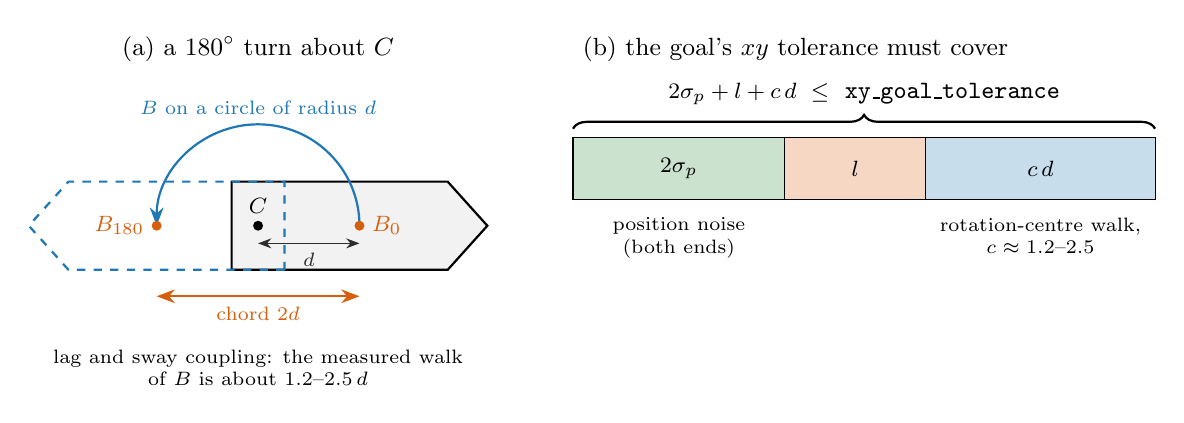
\begin{tikzpicture}[>=Stealth, font=\footnotesize, x=1.12cm, y=1.12cm]
  % ---- (a) an in-place turn about the centre of mass -----------------------------------
  \def\d{1.15}
  \begin{scope}
    \node[font=\small] at (0,2.0) {(a) a $180^\circ$ turn about $C$};
    % hull before (solid) and after (dashed): base_link B at the hull centre, C a distance d aft
    \draw[thick, fill=sD!12] (\d-1.45,-0.5) -- (\d+1.0,-0.5) -- (\d+1.45,0) -- (\d+1.0,0.5)
      -- (\d-1.45,0.5) -- cycle;
    \draw[thick, dashed, sA] (-\d+1.45,-0.5) -- (-\d-1.0,-0.5) -- (-\d-1.45,0) -- (-\d-1.0,0.5)
      -- (-\d+1.45,0.5) -- cycle;
    \draw[->, thick, sA] (\d,0) arc[start angle=0, end angle=180, radius=\d];
    \fill (0,0) circle (1.8pt) node[above=1pt] {$C$};
    \fill[sB] (\d,0) circle (1.8pt) node[right=1pt, sB] {$B_0$};
    \fill[sB] (-\d,0) circle (1.8pt) node[left=1pt, sB] {$B_{180}$};
    \draw[<->, sD!30!black] (0,-0.2) -- node[below, font=\scriptsize] {$d$} (\d,-0.2);
    \draw[<->, sB, thick] (-\d,-0.8) -- node[below, font=\scriptsize] {chord $2d$} (\d,-0.8);
    \node[sA, font=\scriptsize, anchor=south] at (0,\d) {$B$ on a circle of radius $d$};
    \node[font=\scriptsize, align=center, anchor=north] at (0,-1.3)
      {lag and sway coupling: the measured walk\\ of $B$ is about $1.2$--$2.5\,d$};
  \end{scope}
  % ---- (b) the xy tolerance budget ----------------------------------------------------
  \begin{scope}[xshift=4.0cm]
    \node[font=\small, anchor=west] at (0,2.0) {(b) the goal's $xy$ tolerance must cover};
    \draw[fill=sC!25] (0,0.3) rectangle (2.4,1.0);
    \draw[fill=sB!25] (2.4,0.3) rectangle (4.0,1.0);
    \draw[fill=sA!25] (4.0,0.3) rectangle (6.6,1.0);
    \node at (1.2,0.65) {$2\sigma_p$};
    \node at (3.2,0.65) {$l$};
    \node at (5.3,0.65) {$c\,d$};
    \node[font=\scriptsize, align=center, anchor=north] at (1.2,0.2) {position noise\\ (both ends)};
    \node[font=\scriptsize, align=center, anchor=north] at (5.3,0.2) {rotation-centre walk,\\ $c \approx 1.2$--$2.5$};
    \draw[decorate, decoration={brace, amplitude=5pt}, thick] (0,1.1) -- (6.6,1.1)
      node[midway, above=5pt] {$2\sigma_p + l + c\,d \ \le\ $ \code{xy\_goal\_tolerance}};
  \end{scope}
\end{tikzpicture}
\caption{The rotation-centre offset. (a) The hull turns about its centre of mass $C$, but
the controller holds \code{base\_link} $B$, a distance $d$ away, so an in-place turn of
$180^\circ$ carries $B$ along a circle of radius $d$, a chord of $2d$. The velocity lag and
the sway the turn couples in make the walk actually seen about $1.2$--$2.5\,d$. For
$d = 0.10$\,m an ad hoc Python-plant run (\code{t3}/\code{t5}, not a study row) walked
$B$ 0.156\,m at $\omega_z = 0.3$\,rad/s and 0.25\,m at 0.8\,rad/s; the frozen study rows
(\code{com\_aft10}, \code{com\_port5}, seed~0) record only the turn's skid. (b) The $xy$ goal
tolerance must hold the position noise at both ends, $2\sigma_p$, the term $l$ and the
walk $c\,d$. Proportions illustrative.}
\label{fig:spin}
\end{figure}

\file{mhseals\_testing analysis/characterization.py (rule\_limits, nav2\_profile), config/characterize.yaml (nav2\_rules)}

\section{Noise robustness}
\label{sec:noise}

Afloat, every odometry sample carries sensor noise and wave motion: the per-sample neutral SD
$\sigma_f$ that Characterize's neutral phase measures (the wave floor). Two layers pass it on:
MPPI turns it into command chatter, and the velocity loop turns it into thruster reversals.
They are told apart by where the chatter shows: \code{cmd\_chatter\_hz} on \code{/cmd\_vel\_nav}
is MPPI's, \code{thruster\_chatter\_hz} on the pulse widths is the velocity loop's
(Section~\ref{sec:quality}).

\subsection{MPPI: blend more samples, sample closer}
Each cycle MPPI draws $K = 600$ control sequences around its previous plan, perturbed with
standard deviations $\Sigma = \operatorname{diag}(\sigma_{v_x}, \sigma_{v_y}, \sigma_{w_z})$, scores
each by its critics' cost $S_k$ from the current state, and averages them with weights
\[
  w_k = \frac{\exp\!\big(-(S_k - S_\text{min})/\lambda\big)}{\sum_j \exp\!\big(-(S_j - S_\text{min})/\lambda\big)},
  \qquad \bm u \leftarrow \sum_k w_k\,\bm u_k ,
\]
with $\lambda$ the \code{temperature}. The update is a weighted mean of perturbations of size
$\Sigma$, so its spread from cycle to cycle is about $\Sigma/\sqrt{N_\text{eff}}$, with the
effective sample count $N_\text{eff} = 1/\sum_k w_k^2$. At a low temperature $N_\text{eff}$ is
close to 1: the plan follows the single best sample, and when a noisy state sample reorders the
costs, the best sample jumps. Two keys damp that: a higher $\lambda$ raises $N_\text{eff}$, and a
smaller $\Sigma$ shrinks each perturbation. The price is exploration: a plan that moves less per
cycle answers a real change later. Each $\sigma$ stays below its axis limit so samples are not
clipped.

\paragraph{Evidence.} Crane\_ml pair runs, odometry velocity noise 0.05\,m/s, 3 seeds
(Table~\ref{tab:noise}). N1 ($\lambda$ 0.1$\to$0.3, $\Sigma$ $(0.15, 0.10, 0.25)\to(0.10, 0.07, 0.15)$)
cut command chatter 0.28$\to$0.11\,Hz and yaw reversals 4.4$\to$2.1\,/min at the same goal time,
and is the cleanest calm configuration; it is adopted. It does not fix thruster chatter, which
rose to 1.04\,Hz: that is the velocity loop's.

\begin{table}[h]
\centering\small
\begin{tabular}{@{}lccccc@{}}
\toprule
Configuration & goal time & yaw rev/min & cmd chatter & thruster chatter & path ratio \\
\midrule
A1 calm          & 54.0\,s & 3.3 & 0.26\,Hz & 0.16\,Hz & 1.16 \\
N1 calm          & 54.6\,s & 2.0 & 0.11\,Hz & 0.08\,Hz & 1.13 \\
A1 + noise       & 55.6\,s & 4.4 & 0.28\,Hz & \textbf{0.66\,Hz} & 1.20 \\
N1 + noise       & 56.6\,s & 2.1 & 0.11\,Hz & \textbf{1.04\,Hz} & 1.14 \\
A1 + $k_p{\times}0.5$ + noise & 59.8\,s & 3.9 & 0.30\,Hz & 0.40\,Hz & 1.24 \\
N1 + $k_p{\times}0.5$ + noise & 76.3\,s & 0.9 & 0.13\,Hz & 0.38\,Hz & \textbf{1.66} \\
\bottomrule
\end{tabular}
\caption{Noise variants on crane\_ml pair\_test, medians of seeds 0--2 \ev{tune\_P4p\_*; A1 calm: tune\_A1\_pair}.
Bold: fails its threshold (thruster chatter $\le 0.5$\,Hz, path ratio $\le 1.3$).}
\label{tab:noise}
\end{table}

\subsection{The velocity loop: keep noise under the deadband}
The PI term passes odometry noise straight to the effort: per sample its SD is $k_p\sigma_f$.
A thruster reverses only when its effort crosses the ESC deadband $\Delta_e = 25/400 = 0.0625$.
Holding the passed-on noise to half the deadband, the same factor of two as every threshold
against its noise, gives
\[
  k_p \le \frac{\Delta_e}{2\,\sigma_f}.
\]
At $\sigma_f = 0.05$\,m/s that is $k_p \le 0.63$, under today's 0.8, and the crane runs show the
chatter that predicts. In the Python plant's field mix (velocity noise 0.04, waves 0.06) halving
$k_p$ halves thruster reversals, 58.2$\to$28.2\,/min, for 3\% of route time
\ev{noise\_v1:kp1.0\_ki1.0, kp0.5}; halving the nav heading gain instead cuts yaw reversals
21.8$\to$14.2\,/min \ev{noise\_v1:kyaw0.5}. Under MPPI, $k_p\times0.5$ fixes the chatter with A1 but
makes N1 sluggish (Table~\ref{tab:noise}), so the next candidate is $k_p\times0.7$ with N1. A
velocity-loop gain is the hardware owner's change: the procedure proposes it, with this
evidence, and never applies it.

\begin{figure}[tbp]
\centering
\begin{tikzpicture}
\begin{groupplot}[group style={group size=2 by 1, horizontal sep=1.7cm},
  width=0.47\linewidth, height=5.2cm, xmin=-0.08, xmax=1.08, ymin=0,
  xlabel={velocity $k_p$ factor ($\times$ 0.8, 0.8, 0.6)}, xtick={0,0.25,0.5,1},
  xticklabels={0, 0.25, 0.5, 1},
  tick label style={font=\footnotesize}, label style={font=\small},
  legend cell align=left,
  legend style={font=\footnotesize, draw=none, fill=white, fill opacity=0.85, text opacity=1,
    at={(0.03,0.97)}, anchor=north west},
  grid=major, grid style={gray!20}]
\nextgroupplot[ylabel={thruster reversals (/min)}, ymax=72]
  \addplot[sA, thick, mark=*, error bars/.cd, y dir=both, y explicit]
    table[x=kp, y=thr, y error minus=thrlo, y error plus=thrhi] {figures/tuning/data/noise_kp.dat};
  \addlegendentry{$k_{\text{yaw}} = 1$}
  \addplot[sB, only marks, mark=triangle*, mark size=2.8pt, error bars/.cd, y dir=both, y explicit]
    table[x expr=\thisrow{kp}+0.04, y=thr, y error minus=thrlo, y error plus=thrhi] {figures/tuning/data/noise_kyaw.dat};
  \addlegendentry{$k_{\text{yaw}} = 0.5$}
  \addplot[sD, thick, densely dotted, forget plot] table[x=kp, y=thr] {figures/tuning/data/noise_calm.dat};
  \node[font=\scriptsize, sD!30!black, anchor=south east] at (axis cs:1.06,5.09) {calm, no noise};
  \node[font=\scriptsize, anchor=south west] at (axis cs:-0.05,8.5) {f.-f.\ only};
\nextgroupplot[ylabel={route yaw reversals (/min)}, ymax=30]
  \addplot[sA, thick, mark=*, error bars/.cd, y dir=both, y explicit]
    table[x=kp, y=yaw, y error minus=yawlo, y error plus=yawhi] {figures/tuning/data/noise_kp.dat};
  \addplot[sB, only marks, mark=triangle*, mark size=2.8pt, error bars/.cd, y dir=both, y explicit]
    table[x expr=\thisrow{kp}+0.04, y=yaw, y error minus=yawlo, y error plus=yawhi] {figures/tuning/data/noise_kyaw.dat};
  \addplot[sD, thick, densely dotted] table[x=kp, y=yaw] {figures/tuning/data/noise_calm.dat};
  \node[font=\scriptsize, sD!30!black, anchor=south east] at (axis cs:1.06,2.18) {calm, no noise};
\end{groupplot}
\end{tikzpicture}
\caption{Odometry noise through the velocity gain, on the field mix of noise\_v1 (dead time
0.05\,s, odometry latency 0.1\,s, velocity noise 0.04\,m/s, \code{wave\_sd} 0.06); points are the mean
of seeds 0--2, bars the min--max. Left: thruster reversals scale with $k_p$, 58.2, 28.2 and
13.5 per minute at $\times 1$, $\times 0.5$ and $\times 0.25$, and 6.3 with feed-forward only
($k_p = 0$, $k_i$ halved), against 5.09 in calm water. Right: yaw reversals
change less with $k_p$ and spread widely across seeds (21.8, 17.4, 17.1, 11.5 at $\times 1$,
$\times 0.5$, $\times 0.25$, 0); halving Nav2's $k_{\text{yaw}}$ (triangles, offset right)
gives 14.2 at $\times 1$ and 13.1 at $\times 0.5$ and leaves the thruster reversals with
$k_p$ (55.1, 24.7). The rule $k_p \le \Delta e / (2\sigma_f)$, $\Delta e = 0.0625$, keeps the
effort a $2\sigma_f$ velocity-noise excursion produces within one effort step; with the
mix's $\sigma_f = 0.04$\,m/s alone it allows $k_p \le 0.78$, about the $\times 1$ surge gain 0.8. Data:
\code{figures/tuning/data/noise\_*.dat}.}
\label{fig:noise}
\end{figure}

\file{mhseals\_nav config/nav2\_params.yaml (FollowPath temperature, *\_std); mhseals\_hardware config/default.yaml (controller.kp)}

\section{Motion-quality metrics}
\label{sec:quality}

A run is scored from its bag: the truth pose and twist (crane\_ml's \code{/crane/odom},
rigidly aligned into the odometry frame; \code{/odom/local} on the boat), \code{/cmd\_vel\_nav},
the pulse widths and the plan's endpoint as the goal. Most metrics count sign changes with
hysteresis: for a signal $x$ and band $h$, the sign state is set to $\sgn x$ only when $|x| > h$, and
a \emph{reversal} is a change of that state. While the boat is not under way ($|\bm v| \le 0.05$\,m/s
and $|r| \le h$) the state is cleared, so a stop is never a reversal.

\begin{table}[h]
\centering\small
\begin{tabular}{@{}p{0.2\linewidth}p{0.6\linewidth}c@{}}
\toprule
Metric & Definition & pass \\
\midrule
yaw reversals & reversals of the truth yaw rate, $h = 0.05$\,rad/s, per under-way minute & $\le 6$\,/min \\
shake index & the subset whose ended lobe peaked above 0.10\,rad/s and lasted under 4\,s & $\le 1$\,/min \\
command chatter & worst axis of \code{/cmd\_vel\_nav}: reversals with $h = 0.02$ per second & $\le 0.3$\,Hz \\
thruster chatter & worst thruster: sign changes of $p - 1500$ outside $\pm25\,\mu$s, per second & $\le 0.5$\,Hz \\
jerk & RMS planar jerk of the truth, after a 0.2\,s centred moving average & $\le 0.5$\,m/s$^3$ \\
spin in place & time with $|r| > 0.15$\,rad/s and $|\bm v| < 0.05$\,m/s or turn radius $|\bm v|/|r| < 0.4$\,m & report \\
away-spins & in-place turns that rotate away from the goal yaw & $0$ \\
goal overshoot & worst distance past a goal along its approach, after first within 0.4\,m & $\le 0.3$\,m \\
path ratio & worst leg's truth path length over the straight line from leg start to goal & $\le 1.3$ \\
energy & $\int\sum_i |f_i|\,\dd t$ with $f = F^{\pm} e|e|$, $e = (p - 1500)/400$ & report \\
stalls & \code{/cmd\_vel\_nav} gaps over 0.5\,s while a goal is active & $0$ \\
\bottomrule
\end{tabular}
\caption{Motion-quality metrics and their pass thresholds (\code{motion\_quality.yaml}). A goal
leg starts when the plan's endpoint jumps by 0.5\,m; a leg settles when the boat stays within
0.4\,m for 3\,s.}
\label{tab:quality}
\end{table}

\noindent Two choices need a reason. The spin fraction is report-only because a commanded
turn-around (pair\_test, the docking back-out) is a legitimate in-place turn, 11--13\% of every calm
A0, A1 and N1 crane pair run; the gate is away-spins, which are never commanded. And each hysteresis band sits at least twice above the noise of its channel, so noise alone
counts nothing: the yaw band 0.05\,rad/s is over twice the 0.02\,rad/s gyro noise of the field
mix, and a thruster reversal counts only outside the ESC deadband. On the boat the bands are
checked against the measured $\sigma_f$ and $\sigma_r$ before any score is read.

Each metric points at one layer. Command chatter is MPPI's; thruster chatter with clean
commands is the velocity loop's; yaw reversals with clean commands and clean thrusters are delay
(Section~\ref{sec:latency}); goal overshoot and path ratio with clean signals are limits and
tolerances (Section~\ref{sec:limits}).
\file{crane\_ml Tools/Tuning/motion\_quality.py, motion\_quality.yaml; away-spins: navmetrics.py}

\section{Verification in simulation}
\label{sec:verify}

Verification has two stages with different jobs. The Python plant ranks causes in seconds per
run but has no MPPI; crane\_ml runs the whole stack (Nav2, the velocity loop, the mixer, the
physics player) and is the only stage that confirms a Nav2 change.

\subsection{Stage 1: the Python plant matrices}
\code{study.py} runs a matrix file against the plant of Section~\ref{sec:plant} with the boat's
velocity law and mixer imported unchanged. Each JSONL row holds the variant, the limits, the
seed, a case hash and the git heads, and \code{rerun(row)} reproduces it alone.

\begin{center}\small
\begin{tabular}{@{}llp{0.55\linewidth}@{}}
\toprule
Matrix & rows & varies \\
\midrule
\code{plant\_v1} & 26 cases, seed 0 & mass, inertia, added mass, CoM, drag, thrust scale, sag, reverse ratio, mount error, ESC deadband, spin-up, dead time, latency; five of them also uncharacterized \\
\code{disturb\_v1} & 23 cases, seeds 0--2 & current, wind, waves, velocity noise, latency, GPS $\sigma$ and float, heading bias, dead thruster, field mix \\
\code{noise\_v1} & 9 cases, seeds 0--2 & velocity $k_p$, $k_i$, nav heading and position gains in the field mix \\
\code{rules\_v1} & 6 cases, seeds 0--2 & today's limits against the rule caps, calm, field mix, heavy \\
\code{stale\_drift\_v1} & 6 cases, seeds 0--2 & observer on/off, \code{integral\_limit}, current 0.3 and 0.45\,m/s \\
\bottomrule
\end{tabular}
\end{center}

\paragraph{Metamorphic relations.} The boat's true parameters are unknown, so the plant matrix
checks relations between runs instead of values against truth:
\begin{enumerate}[leftmargin=*, itemsep=1pt]
\item \emph{Absorption}: a characterized steady plant change (mass, drag, thrust, reverse ratio,
  mount) moves route time by at most $\pm5\%$ and adds no failed goal. Holds in \code{plant\_v1}
  ($\pm3\%$).
\item \emph{Monotone in delay}: more dead time or latency never lowers the yaw step overshoot
  (0.10, 0.40, 0.82 at dead time 0, 0.15, 0.3\,s; 0.58 at 0.2\,s latency \ev{plant\_v1}).
\item \emph{Monotone in noise}: more velocity noise or wave SD never lowers thruster reversals
  (5.1, 30.6, 152\,/min at 0, 0.05, 0.12\,m/s; 8.0, 24.2 for waves 0.05, 0.12 \ev{disturb\_v1}).
  Yaw reversals are not monotone in noise (waves 0.05: 1.7\,/min against 2.2 calm), so no relation
  is drawn on them.
\item \emph{Layer separation}: a velocity-loop gain change moves thruster reversals far more than
  command chatter, and a nav gain change the reverse (\code{noise\_v1}).
\end{enumerate}
A violated relation is a finding about the stack, not noise to average away.

\subsection{Stage 2: crane\_ml full stack}
The candidate is a Nav2 YAML on \code{tuning-nav} built into an overlay; the baseline is
origin/main. Each cell runs \code{pair\_test} (goal behaviour) and the full \code{mission} task, 3
seeds calm and 2 per disturbance, at most 3 instances machine-wide, \code{nice -n 10}, backing
off above 85\,$^\circ$C. Every session records the seed, the player commit, the overlay and
parameter hashes and the git heads.

\begin{center}\small
\begin{tabular}{@{}lp{0.68\linewidth}@{}}
\toprule
Axis & cells \\
\midrule
disturbance & calm; current 0.2\,m/s at 90$^\circ$; wind 5\,m/s at 45$^\circ$; GPS $\sigma$ 0.3\,m; odometry velocity $\sigma$ 0.05\,m/s \\
plant (faults player) & mass 19 / 40\,kg; CoM aft / port; reverse ratio 0.6; weak / dead FL; dead time 0.2\,s; spin-up 0.3\,s \\
\bottomrule
\end{tabular}
\end{center}

\paragraph{What it has shown.} In pair runs (Table~\ref{tab:pair}) turning to the goal yaw inside
the tolerance (A1) is the one clear win; widening the rotation shim's threshold (A2) and the yaw
caps alone (A3) are not accepted. The full mission adds failures no pair run sees, and each was
traced to one layer before anything was tuned: the dock pin to the drift observer
(Section~\ref{sec:observer}); a back-out goal 2.9\,rad behind the boat, over the shim's 1.8\,rad
threshold, turning in the bay (fixed in the task by a straight back-up); a speed lap ending 1\,s
after it started on the previous goal's success (fixed by resending a success that arrives early
and far from the route end); and buoy contacts between offset gates, still open, where MPPI's
cost critic weight (3.81) is low against the path critics (10). Full-mission results from player
\code{bf82744} are invalid (buoys leave detection after about 21\,s) and are not used.

\begin{table}[h]
\centering\small
\begin{tabular}{@{}llccccc@{}}
\toprule
& change against main & goal time & overshoot & yaw rev/min & path ratio & away-spins \\
\midrule
A0 & none & 51.7\,s & 0.24\,m & 5.7 & 1.25 & 0 \\
A1 & \code{rotate\_to\_goal\_heading} & 54.0\,s & 0.02\,m & 3.3 & 1.16 & 0 \\
A2 & A1 + shim threshold 2.6 & 70.9\,s & 0.09\,m & 2.6 & 1.21 & 1 \\
A3 & A1 + $w_z$/$\alpha_z$ 0.42/0.46 & 56.1\,s & 0.06\,m & 4.1 & \textbf{1.32} & 1 \\
\bottomrule
\end{tabular}
\caption{crane\_ml pair\_test, 240\,s, calm, medians of seeds 0--2 \ev{tune\_A\{0,1,2,3\}\_pair*}.
Away-spins are totals over the three seeds. A1 adopted; A2 rejected (one run 0.67\,m overshoot, path ratio 2.43); A3 retested with the full rule
set on the fixed player.}
\label{tab:pair}
\end{table}

\subsection{Acceptance}
\label{sec:accept}
The thresholds are fixed before the runs. A candidate is accepted only if, over the whole matrix:
\begin{enumerate}[leftmargin=*, itemsep=1pt]
\item the mission succeeds in at least 90\% of cells and in every calm cell;
\item the median of every gated metric passes Table~\ref{tab:quality}, with zero away-spins and zero stalls;
\item no metric is worse than the baseline in more than one cell in five;
\item mission time is no worse than the baseline's $+5\%$.
\end{enumerate}
A failure goes back to the step whose layer the failing metric points at
(Section~\ref{sec:quality}), not to the nearest Nav2 key.
\file{crane\_ml Tools/Tuning/study.py, matrices/*.yaml; rig run\_sim.sh, batch.sh}

\section{On the boat: measurements, gates and stopping}
\label{sec:field}

Agents never apply parameters to the boat and never write the FCU. Every boat step is a
proposal the owner executes; the sim steps run unattended. The thrusters stay disconnected and
every step is a dry run (\code{boat\_trial check --profile boat --gate t} clean) until the owner
says otherwise, and arming stays with the owner. Heading and velocity data from the period the
FCU yaw source was wrong are never inputs.

\subsection{What to measure}
\begin{center}\small
\begin{tabular}{@{}p{0.17\linewidth}p{0.25\linewidth}p{0.28\linewidth}p{0.2\linewidth}@{}}
\toprule
Quantity & Session & Analysis & Sets \\
\midrule
mass, CoM, lever arm $l$ & bench (\texttt{bench.pdf}) & --- & URDF, $l$ \\
noise floor $\sigma_f$, $\sigma_r$ & Characterize, neutral phase (20\,s) & neutral noise $\to$ \code{wave\_floor} & $k_p$, stopped velocities \\
dead time $L$ & the same session's yaw onsets & \code{latency.py} (Section~\ref{sec:latency}) & all rules \\
lag $\tau$ per axis & Controller steps, amplitude = planned limit & rise time$/\ln 9$ & all rules \\
offset $d$ & Characterize yaw rows & $|v|/|r|$ on yaw holds, lever-corrected & xy tolerance, rotate speed \\
$\sigma_p$ per fix tier & 5\,min moored per tier & SD of the global position & xy tolerances, docking gate \\
current, wind & Conditions panel & conditions verdict & go / no-go \\
\bottomrule
\end{tabular}
\end{center}

\noindent A fit stands until something says it no longer describes the boat: the
change-point sentinel firing (critical value 4.60, the owner's correction of the sim-to-real review's 4.57), a hardware change, or a
new day's conditions outside those it was fitted in. Then the boat is re-characterized before
any tuning.

\subsection{Gates}
These are not tuned around; each one stops the session or the task.
\begin{itemize}[leftmargin=*, itemsep=1pt]
\item \textbf{Conditions}: current $\le 0.3$\,m/s, wind $\le 6$\,m/s, and a wave floor under 2.5 times the
  one the tuning assumed. Otherwise no tuning run.
\item \textbf{Dead or weak thruster}: a direction Characterize marks dead fails the motion gates
  (the \code{calib.dead} check). No Nav2 tuning that day: the route still completes in simulation, but
  goals overshoot by 0.77\,m \ev{disturb\_v1:FL\_dead}.
\item \textbf{Latency}: $L > 0.3$\,s means fixing the odometry chain first (Section~\ref{sec:latency}).
\item \textbf{Fix tier}: docking and other precise goals start only at RTK fixed; if $\sigma_p$ at the
  session's tier exceeds 0.15\,m, docking is perception-only or skipped.
\item \textbf{Drift}: a drift estimate over 0.35\,m/s keeps precise tasks from starting
  (Section~\ref{sec:observer}). It is a start gate only; a running task is aborted only by
  saturated thrusters off the command.
\end{itemize}

\subsection{Order and stopping}
The runs go in increasing exposure, and the first failure ends the day's tuning:
\[
  \text{Characterize} \to \text{Controller steps} \to \text{Station keeping} \to
  \text{Waypoint square} \to \text{single tasks} \to \text{mission}.
\]
Nav2 keys that apply live go through \code{boat\_trial config apply nav2 --yes}, which writes the
overlay first; keys that need a restart trigger a Navigation reset. Velocity-loop gains are the
hardware owner's change.

\paragraph{Abort.} Thruster chatter over 2\,Hz, yaw reversals over 15\,/min or a goal overshoot over
1\,m (four, two and a half, and over three times their pass thresholds): abort the task, release the hold, and
revert to the last good overlay. A hold puts the thrusters in neutral (Section~\ref{sec:observer});
the RC mode switch takes over at any time; the remote e-stop cuts thruster power.

\paragraph{Decide.} A field change is kept only if its session passes the metrics of
Section~\ref{sec:quality} computed from \code{/odom/local} with the bands checked against the day's
$\sigma_f$, and is no worse than the last good overlay on the same course. Otherwise it is reverted
and the failing metric's layer is the next thing to look at, back in simulation.
\file{mhseals\_testing boat\_test procedures (Characterize, Controller steps), harness gates; mhseals\_nav task conditions}


\appendix
\section{Evidence index}
\label{app:evidence}

Every bracketed citation names one of the sources below. Python-plant rows re-run alone with
\code{study.rerun(row)}; the plotted rows are frozen under \code{docs/figures/tuning/study/} and
the figures regenerate with \code{make tuning-figures}.

\begin{center}\small
\begin{tabular}{@{}p{0.3\linewidth}p{0.64\linewidth}@{}}
\toprule
Citation & Source \\
\midrule
\ev{plant\_v1:\textit{case}} & Python plant, \code{matrices/plant\_v1.yaml}, seed 0, row \textit{case} \\
\ev{disturb\_v1}, \ev{noise\_v1}, \ev{rules\_v1}, \ev{stale\_v1} & Python plant, the matrix of that name (\code{stale\_drift\_v1.yaml} for \code{stale\_v1}), seeds 0--2 \\
\ev{latency synthetic} & 16 synthetic onsets (dead time 0--0.3\,s, spin-up 0.1/0.25\,s, odometry latency 0/0.1\,s) through \code{latency.estimate} \\
\ev{crane relay latency fit} & crane\_ml Characterize yaw onsets with \code{pwm\_relay.py} dead time 0 and 0.1\,s, 8 onsets each \\
\ev{tune\_A\textit{n}\_pair} & crane\_ml pair\_test sessions, 240\,s, seeds 0--2, scored by \code{motion\_quality.py} and \code{navmetrics.py} \\
\ev{tune\_P4p\_*} & crane\_ml pair\_test, odometry velocity $\sigma$ 0.05, seeds 0--2 \\
\ev{ma\_v2}, \ev{ma\_v3} & crane\_ml full-mission batches of the mission-autonomy branch (rig-percep player) \\
\ev{sim2real R\textit{n}} & the sim-to-real specification's adversarial-review verdict table (\S17); only confirmed or plausible claims are cited, and R3-8 only for its corrected sign \\
\ev{ad hoc runs t3/t5} & throwaway Python-plant scripts (in-place turns with a CoM offset), not a study matrix; their numbers are estimates \\
\bottomrule
\end{tabular}
\end{center}

\noindent Python-plant numbers rank causes; they are not boat numbers, and none of them confirms a
Nav2 change without a crane\_ml run. The nominal plant is crane\_ml's physics, a fixture.


\end{document}
